\chapter{Datenstrukturen}
\label{chp:Containers}
\epigraph{
	Multimedia? As far as I'm concerned, it's reading with the radio on!
}{Rory Bremmer}

Bis hierhin haben wir sehr kleine Datenmengen behandelt. Unser bisheriges \enquote{Arbeitsmaterial} waren
Variablen, die je einen einzelnen Wert repräsentieren. Eine Stärke von Computern ist es aber gerade, große
Datenmengen schnell zu verarbeiten. Hier werden wir Möglichkeiten kenenn lernen, nahezu beliebig
große Datenmengen im Speicher zu halten und zu manipulieren.

\section{Speichermodell}
\label{sec:MemoryModel}
Bevor wir das Verhalten der verschiedenen Speicherstrukturen verstehen können, die Python uns zur Verfügung stellt, müssen wir uns mit der Art und Weise vertraut machen, in der Daten im Speicher abgelegt werden.

Man kann sich den Arbeitsspeicher als langes Band von kleinen, nummerierten Speicherzellen vorstellen. Jede Zelle fässt genau ein Byte. Um einen Wert zu lesen oder zu schreiben muss dem Prozessor die Nummer der Zelle mitgeteilt werden, die verändert wird. Diese Nummer wird \emph{Adresse} oder \emph{Pointer} genannt. Wenn wir im Code Variablen benutzen, übersetzt der Compiler diese in Adressen. 

\begin{tcolorbox}[title=Speicherbild]
\begin{center}
\begin{tikzpicture}
  [ 
    cell/.style={text width=8mm,
      text height=4mm, draw=black, inner sep=1mm},
    ld/.style={draw=blue,shorten >=2pt,->}
  ]
  \node (c1) at (0,0) [cell] {\ttfamily 99};
  \node (c2) at (1,0) [cell] {\ttfamily 1};
  \node (c3) at (2,0) [cell] {\ttfamily 255};
  \node (c4) at (3,0) [cell] {\ttfamily 0};
  \node (c5) at (4,0) [cell] {\ttfamily 80};
  \node (c6) at (5,0) [cell] {\ttfamily ...};

  \node (labelMem) at (8,  1) {Symbole im Code};
  \node (labelMem) at (8,  0) {Werte im Speicher};
  \node (labelMem) at (8, -1) {Adressen};
  
  \node (a1) [below=2mm of c1]             {\tiny 0x27ff};
  \node (a2) [below=2mm of c2, color=teal] {\tiny 0x2800};
  \node (a3) [below=2mm of c3]             {\tiny 0x2801};
  \node (a4) [below=2mm of c4]             {\tiny 0x2802};
  \node (a5) [below=2mm of c5]             {\tiny 0x2803};
  \node (a6) [below=2mm of c6]             {\tiny 0x2804};
  
  \node (ptr) [below=8mm of c1] {\scriptsize Adresse von \texttt{x}};
  \node (vc2) [above=6mm of c1] {\scriptsize Variable \texttt{x}};
  \node (vc0) [above=2mm of c1] {\scriptsize Variable \texttt{y}};
  
  \draw [ld, teal] (ptr.east) .. controls +(0.3,0) .. (a2.south);
  \draw [ld]       (vc0.east) .. controls +(0.4,0) .. (c2.north);
  \draw [ld]       (vc2.east) .. controls +(2.4,0) .. (c4.north);
\end{tikzpicture}
\end{center}
\end{tcolorbox}
{\captionof{figure}{Speicherbild: nummerierte Zellen}}

Während wir der Einfachheit halber oft sagen, dass eine Variable einen \emph{Wert} speichert, ist tatsächlich die Information hinterlegt, \emph{wo der Wert selbst zu finden ist}, also die Adresse des Wertes. Dies hat den Vorteil, dass Aufgaben sehr effizient erledigt werden können, wenn große Datenmengen bewegt werden müssen: anstatt viele Megabytes zu kopieren, muss nur eine Referenz an die Stelle gesetzt werden, wo die zu kopierenden Daten bereits im Speicher liegen. Für uns als ProgrammiererInnen heißt dies aber auch, dass wir diese Speicherstruktur im Hinterkopf behalten müssen.

Stellen Sie sich vor, Sie verwalten eine Liste. Diese soll über den Variablennamen \inPy{originalList} ansprechbar sein. Nun wollen Sie eine Arbeitskopie dieser Liste anlegen und \emph{in dieser Kopie} Werte verändern. Sie wollen also folgendes Speicherbild erreichen:

\begin{tcolorbox}[title=Speicherbild]
\begin{center}
\begin{tikzpicture}
  [ 
    cell/.style={text width=8mm,
      text height=4mm, draw=black, inner sep=1mm},
    ld/.style={draw=blue,shorten >=2pt,->}
  ]
  \node (gap1) at ( 0,0)        {\ttfamily ...};
  \node (v1)   at ( 1,0) [cell] {\ttfamily 1};
  \node (v2)   at ( 2,0) [cell] {\ttfamily 2};
  \node (v3)   at ( 3,0) [cell] {\ttfamily 3};
  \node (v4)   at ( 4,0) [cell] {\ttfamily 4};
  \node (gap2) at ( 5,0)        {\ttfamily ...};
  \node (c1)   at ( 6,0) [cell] {\ttfamily 1};
  \node (c2)   at ( 7,0) [cell] {\ttfamily 2};
  \node (c3)   at ( 8,0) [cell] {\ttfamily 3};
  \node (c4)   at ( 9,0) [cell] {\ttfamily 4};
  \node (gap3) at (10,0)        {\ttfamily ...};
  
  \draw [decorate, decoration={brace,amplitude=7pt}, xshift=-0pt, yshift=0pt]
  		( 0.75, 0.5) -- ( 4.25, 0.5) node [midway, yshift=+0.5cm] 
		(braceArrayPreResize) {Originaldaten};
  \draw [decorate, decoration={brace,amplitude=7pt}, xshift=-0pt, yshift=0pt]
  		( 5.75, 0.5) -- ( 9.25, 0.5) node [midway, yshift=+0.5cm] 
		(braceArrayPreResize) {Arbeitskopie};

  \node (a1) [below=2mm of v1, color=teal] {\tiny 0x2800};
  \node (a2) [below=2mm of v2]             {\tiny 0x2801};
  \node (a3) [below=2mm of v3]             {\tiny 0x2802};
  \node (a4) [below=2mm of v4]             {\tiny 0x2803};
  
  \node (b1) [below=2mm of c1, color=teal] {\tiny 0x2950};
  \node (b2) [below=2mm of c2]             {\tiny 0x2951};
  \node (b3) [below=2mm of c3]             {\tiny 0x2952};
  \node (b4) [below=2mm of c4]             {\tiny 0x2953};
  
  \node (p1) [below=8mm of gap1] {\scriptsize Adresse von \texttt{originalList}};
  \node (p2) [below=8mm of gap2] {\scriptsize Adresse von \texttt{copyOfList}};

  \draw [ld, teal] (p1.east) .. controls +(0.3,0) .. (a1.south);
  \draw [ld, teal] (p2.east) .. controls +(0.3,0) .. (b1.south);
\end{tikzpicture}
\end{center}
\end{tcolorbox}
{\captionof{figure}{Speicherbild: Arbeitskopie}}

Wenn Sie nun die Codezeile
\begin{center}
	\inPy{copyOfList = originalList}
\end{center}
tippen, werden Sie aufgrund dieser Arbeitsweise von Python aber folgendes Speicherbild erzeugen:

\begin{tcolorbox}[title=Speicherbild]
\begin{center}
\begin{tikzpicture}
  [ 
    cell/.style={text width=8mm,
      text height=4mm, draw=black, inner sep=1mm},
    ld/.style={draw=blue,shorten >=2pt,->}
  ]
  \node (gap1) at ( 0,0)        {\ttfamily ...};
  \node (v1)   at ( 1,0) [cell] {\ttfamily 1};
  \node (v2)   at ( 2,0) [cell] {\ttfamily 2};
  \node (v3)   at ( 3,0) [cell] {\ttfamily 3};
  \node (v4)   at ( 4,0) [cell] {\ttfamily 4};
  \node (gap2) at ( 5,0)        {\ttfamily ...};
  \node (c1)   at ( 6,0) [cell] {\ttfamily 19};
  \node (c2)   at ( 7,0) [cell] {\ttfamily 89};
  \node (c3)   at ( 8,0) [cell] {\ttfamily 3};
  \node (c4)   at ( 9,0) [cell] {\ttfamily 29};
  \node (gap3) at (10,0)        {\ttfamily ...};
  
  \draw [decorate, decoration={brace,amplitude=7pt}, xshift=-0pt, yshift=0pt]
  		( 0.75, 0.5) -- ( 4.25, 0.5) node [midway, yshift=+0.5cm] 
		(braceArrayPreResize) {Originaldaten};
  \draw [decorate, decoration={brace,amplitude=7pt}, xshift=-0pt, yshift=0pt]
  		( 5.75, 0.5) -- ( 9.25, 0.5) node [midway, yshift=+0.5cm] 
		(braceArrayPreResize) {andere Daten};

  \node (a1) [below=2mm of v1, color=teal] {\tiny 0x2800};
  \node (a2) [below=2mm of v2]             {\tiny 0x2801};
  \node (a3) [below=2mm of v3]             {\tiny 0x2802};
  \node (a4) [below=2mm of v4]             {\tiny 0x2803};
  
  \node (b1) [below=2mm of c1]             {\tiny 0x2950};
  \node (b2) [below=2mm of c2]             {\tiny 0x2951};
  \node (b3) [below=2mm of c3]             {\tiny 0x2952};
  \node (b4) [below=2mm of c4]             {\tiny 0x2953};
  
  \node (p1) [below=8mm of gap1] {\scriptsize Adresse von \texttt{originalList}};
  \node (p2) [below=8mm of gap2] {\scriptsize Adresse von \texttt{copyOfList}};

  \draw [ld, teal] (p1.east) .. controls +( 0.3,0) .. (a1.south);
  \draw [ld, red ] (p2.west) .. controls +(-0.3,0) .. (a1.south);
\end{tikzpicture}
\end{center}
\end{tcolorbox}
{\captionof{figure}{Speicherbild: Zwei Referenzen auf dieselben Daten}}

Anstatt eine Kopie der Liste anzulegen, haben Sie nur eine \emph{Kopie der Referenz} erzeugt. Ein Zugriff über das Symbol \inPy{copyOfList} ändert also immer noch Ihr Original!

Um nun das gewünschte Ziel zu erreichen, müssen Sie stattdessen die Funktion \inPy{copy} aus dem Modul \inPy{copy} benutzen:

\begin{codebox}[Schema: Shallow Copy anlegen]
\begin{minted}{python3}
import copy

# Code zum Aufbau der Liste originalList

copyOfList = copy.copy(originalList)
\end{minted}
\end{codebox}

\section{mutable und immutable objects}
Python kennt zwei große Gruppen von Objekten: veränderbare Objekte (\emph{mutable objects}) und unveränderliche Objekte (\emph{immutable objects}).

Die \emph{Werte} von immutable objects dürfen sich nicht mehr ändern, sobald sie einmal im Speicher abgelegt wurden. Wenn eine Variable geändert wird, die ein immutable object speichert, so wird ein neues Objekt im Speicher konstruiert, nicht aber die alte Stelle überschrieben.

Betrachten Sie dazu das folgende Beispiel:

\begin{codebox}[Codebeispiel, width=.495\linewidth, on line, equal height group=immutableEvolutionGroup]
\begin{minted}[linenos]{python3}
# int-Variablen sind immutable

intVar = 100

intVar = 200
\end{minted}
\end{codebox}
%
\begin{tcolorbox}[title=Speicherbild,
	width=.495\linewidth,
	on line,
	equal height group=immutableEvolutionGroup]
\begin{tikzpicture}
  [ 
    cell/.style={text width=8mm,
      text height=4mm, draw=black, inner sep=1mm},
    ld/.style={draw=blue,shorten >=2pt,->}
  ]
  \node (gap1) at ( 0,0)        {\ttfamily ...};
  \node (v1)   at ( 1,0) [cell] {\ttfamily 100};
  \node (v2)   at ( 2,0) [cell] {\ttfamily 2};
  \node (v3)   at ( 3,0) [cell] {\ttfamily 3};
  \node (v4)   at ( 4,0) [cell] {\ttfamily 4};
  \node (v5)   at ( 5,0) [cell] {\ttfamily 200};
  \node (gap2) at ( 6,0)        {\ttfamily ...};
  
  \node (a1) [below=2mm of v1] {\tiny 0x2800};
  \node (a2) [below=2mm of v2] {\tiny 0x2801};
  \node (a3) [below=2mm of v3] {\tiny 0x2802};
  \node (a4) [below=2mm of v4] {\tiny 0x2803};
  \node (a5) [below=2mm of v5] {\tiny 0x2804};
  
  \node (p1) [below=8mm of v3] {\scriptsize Adresse von \texttt{intVar}};

  \draw [ld, teal, densely dotted] (p1.west) .. controls +(-0.3,0) .. (a1.south)
  		node (l1) [below=4mm] {\scriptsize bis Zeile 3};
  \draw [ld, blue                ] (p1.east) .. controls +(+0.3,0) .. (a5.south) 
  		node (l1) [below=4mm] {\scriptsize ab Zeile 5};
\end{tikzpicture}
\end{tcolorbox}

In dem hier gezeigten Code ändern wir augenscheinlich den Wert von \inPy{intVar}. Der Typ \inPy{int} ist jedoch immutable! Daher wird der Python-Interpreter dafür sorgen, dass mit Zeile 5 ein neues \inPy{int}-Objekt im Speicher angelegt wird, das den neuen Wert speichert. Die Referenz von \inPy{intVar} geht nun auf diese neue Speicherstelle. Der Wert 100, der in der alten Speicherstelle lag, wird hingegen nicht angerührt.

Bei mutable objects hingegen wird wirklich der Inhalt der Speicherzellen selbst überschrieben. Sie erkennen, dass hier das Problem der vermeintlichen Arbeitskopie auftritt.

Im Moment haben wir nur immutable objects kennen gelernt. In diesem Kapitel werden die ersten mutable objects eingeführt. Am Ende des Kapitels finden Sie eine Übersichtstabelle zu den Ihnen bis dahin bekannten Speicherstrukturen.

\begin{hintbox}[Speicheradresse ausfindig machen mit \texttt{id}]
Der Befehl \inPy{id} kann auf alle Datenobjekte angewandt werden, und gibt die Adresse im Speicher aus, also die Nummer der Speicherzelle.

Neben Variablen (\inPy{id(x)} -- Adresse der Variablen \inPy{x}) kann der Befehl auch auf Datentypen (\inPy{id(int)} -- Adresse der \enquote{Beschreibung des Typs}) und auf Konstanten (\inPy{id(1)} -- Adresse des Werts \inPy{1}) angewandt werden.

Wenn Sie hier ein wenig experimentieren, werden Sie feststellen, dass \enquote{kleine} Ganzzahlen in relativer Nähe zueinander liegen, während \enquote{große Zahlen} (> 256) signifikant andere Adressen erhalten. Dies liegt daran, dass die Entwickler von Python erwartet haben, dass diese Zahlen sehr häufig als (Zwischen-)Ergebnisse auftreten. Daher werden diese bereits \enquote{auf Verdacht vorbereitet}. Größere Zahlen werden erst im Speicher angelegt, wenn dies wirklich nötig wird.
\end{hintbox}

\begin{hintbox}[Vergleichsoperator \texttt{is} vs. \texttt{==}]
Wir haben bereits den Operator \inPy{==} kennengelernt, der uns mitteilt, ob zwei Objekte gleich sind. Hierbei ist mit \emph{Gleichheit} gemeint, dass sie denselben Wert speichern. Wie Sie gesehen haben, können Kopien voneinander an verschiedenen Speicherorten abgelegt werden.

Der Operator \inPy{is} vergleicht nicht die Werte, sondern die Speicheradressen, und gibt folglich \inPy{True} zurück, wenn zwei Variablen dasselbe Objekt referenzieren. Die folgenden beiden Codezeilen sind also äquivalent:
\begin{codebox}[Übersetzung von \texttt{is}]
\begin{minted}{python3}
print( id(a) == id(b) )
print(    a  is    b  )
\end{minted}
\end{codebox}
\end{hintbox}
%
\begin{hintbox}[]
Beachten Sie, dass diese Bedeutung des Operators \inPy{is} manchmal unintuitives Verhalten erzeugt:
\begin{warnbox}[Unintuitives Verhalten von \texttt{is}]
\begin{minted}{python3}
5 == 4 is not True
\end{minted}
\end{warnbox}
dieser Ausdruck wird zu \inPy{True} ausgewertet, obwohl offensichtlich $5 \neq 4$ gilt.

Dies lässt sich folgendermaßen begründen:

Python wertet zunächst den ersten Teil der Aussage (\inPy{5 == 4}) zu \inPy{False} aus. Dieser Wert ist ein häufig gebrauchter, und wurde daher von Python bereits vorbereitet, hatte also schon vor diesem ersten Rechenschritt eine Adresse. Diese Adresse wird dem Ausdruck \inPy{5 == 4} zugeordnet.

Als nächstes wird die zweite Teilaussage (\inPy{not True}) ebenfalls zu \inPy{False} ausgewertet. Wieder erkennt Python den vorbereiteten Wert, und weist \inPy{not True} die Adresse von \inPy{False} zu.

Der Operator \inPy{is} vergleicht nun die Adressen von \inPy{False} und \inPy{False}, und kommt folgerichtig zu dem Ergebnis, dass diese gleich sind. Mit anderen Worten, \inPy{False is False} ist \inPy{True}.
\end{hintbox}


\section{\inPy{list}s}
Der Datentyp \inPy{list} repräsentiert -- wie der Name vermuten lässt -- Listen. Die aufgelisteten Werte können dabei ganz verschiedener Natur sein: \inPy{list}s können \inPy{int}s, \inPy{float}s, \ldots und sogar andere Listen enthalten. Die Elemente derselben Liste müssen nicht vom selben Typ sein.

\subsection{Anlegen und Auslesen}
Erstellt werden Listen, indem man in [eckigen Klammern] die Elemente der Liste durch Kommata getrennt aufzählt:
\begin{codebox}[Syntax: Liste anlegen]
listVariable = [listItem1, listItem2, ...]
\end{codebox}

Listen dürfen auch leer sein. Eine leere Liste wird als \inPy{[]} geschrieben.

Auf die Elemente einer Liste wird mittels ihres \emph{Index} zugegriffen, \ie der Nummer innerhalb der Liste. Dabei hat das erste Element der Liste den Index \inPy{0}! Der Index wird in [eckigen Klammern] dem Symbol der Listenvariable nachgestellt, um anzugeben, dass man ein einzelnes Element der Liste ansprechen will:

\begin{codebox}[Syntax: Listenelement ansprechen]
listVariable[listItems]
\end{codebox}

Indices können auch negativ sein! In diesem Falle wird \enquote{von hinten herein} gezählt. \inPy{-1} referenziert also das letzte Element der Liste, \inPy{-2} das vorletzte, usw.

Ist das referenzierte Listenelement selbst eine Liste, so kann auf dessen Elemente ebenfalls durch Nennung des Index in einer eigenen Klammer zugegriffen werden.

\inPy{list}s können auch in normale Variablen \enquote{entpackt} werden. Dazu verwendet man den Zuweisungsoperator \inPy{=}, gibt aber auf der linken Seite so viele Elemente an, wie sie in der Liste sind:
\begin{cmdbox}[Entpacken von Listen]
\begin{minted}{text}
>>> numbers = [1, 2, 3]
>>> a, b, c = numbers
>>> b
2
\end{minted}
\end{cmdbox}


\subsection{Slicing}
Aus einer Liste kann auch ein Teil herausgegriffen werden. Man nennt dies \emph{slicing}:
\begin{codebox}[Syntax: Slicing]
listVariable[start : end : stride]
\end{codebox}
Mit dieser Syntax wird eine \emph{neue Liste} berechnet, die beim Index \inPy{start} beginnt, die Elemente bis \emph{ausschließlich} dem Index \inPy{end} beinhaltet, und deren Elemente in der Quell-Liste einen Abstand von \inPy{stride} haben. Wird \inPy{stride} ausgelassen, werden alle Elemente zwischen \inPy{start} und \inPy{end} in die neue Liste übernommen.

Wird \inPy{start} oder \inPy{end} ausgelassen, so versteht Python dies als: \enquote{vom Anfang} bzw. als \enquote{bis zum Ende}.

\subsection{Addition und Multiplikation bei Listen}
Die Addition von Listen führt zur Verkettung, wie Sie das schon von Strings kennen. Genauso wie dort führt die Multiplikation mit einer Ganzzahl zu einer \emph{Wiederholung} der Listenelemente:
\begin{cmdbox}[Multiplikation von Listen]
\begin{minted}{text}
>>> [1, 2] + [3]
[1, 2, 3]
>>> 3 * [1, 2]
[1, 2, 1, 2, 1, 2]
\end{minted}
\end{cmdbox}

\subsection{Beispiel}
\begin{codebox}[Beispiel: Listenzugriffe]
\begin{minted}[linenos]{python3}
myList = [1, 2, -5, 3.14, "some text", [3, 2], (1+1j)]

print(myList[0])        # erstes Element
print(myList[-1])       # letztes Element
print(myList[-2][0])    # erstes Element des vorletzten Elements
print(myList[1:3])      # slicing: Elemente 1 und 2 (ausschließlich 3)
print(myList[-2:])      # slicing: vorletztes Element bis Ende
print(myList[:5:2])     # slicing: Elemente mit Indices 0 bis 4 in 2er-Schritten
print(myList[::2])      # slicing: alle mit geradem Index

myList += [[]]          # an die Liste eine leere Liste anhängen
print(myList[-1])       # letztes Element
print(myList)           # gesamte Liste
\end{minted}
\end{codebox}

\begin{cmdbox}[Ausgabe]
\begin{minted}{text}
1
(1+1j)
3
[2, -5]
[[3, 2], (1+1j)]
[1, -5, 'some text']
[1, -5, 'some text', (1+1j)]
[]
[1, 2, -5, 3.14, "some text", [3, 2], (1+1j), []]
\end{minted}
\end{cmdbox}
Beachten Sie besonders die Klammern in Zeile 11: \inPy{myList += [[]]}. Die äußeren Klammern geben an, dass das Objekt, das addiert wird, eine Liste ist. Dies ist notwendig, da nur die Addition zwischen Listen erklärt ist; \inPy{myList += 3} würde (für den Python-Interpreter) keinen Sinn ergeben. Alles, was \emph{in diesen Klammern steht}, wird an die Liste angehängt. In diesem Fall ist dies \inPy{[]}, also eine leere Liste. Machen Sie sich klar, dass im Gegensatz zu \inPy{myList += [[]]} (anhängen einer leeren Liste) durch den Befehl \inPy{myList += []} \emph{nichts} zu \inPy{myList} hinzugefügt wird.

\inPy{list}s sind mutable. Das heißt, für Kopien muss der \inPy{copy}-Befehl aus dem Modul \inPy{copy} verwendet werden, oder mittels der Slicing-Syntax eine Kopie erstellt werden:
\begin{codebox}[Beispiel: mutable list]
\begin{minted}[linenos]{python3}
import copy

originalList = [1, 2, 3]
refCopy = originalList
truCopy = copy.copy(originalList)
altCopy = originalList[:]

refCopy += [4]
truCopy += [5, 5]
altCopy += [6, 6]

print("original    : ", originalList)
print("copy.copy   : ", truCopy)
print("slicing copy: ", altCopy)
\end{minted}
\end{codebox}

\begin{cmdbox}[Ausgabe]
\begin{minted}{text}
original    : [1, 2, 3, 4]
copy.copy   : [1, 2, 3, 5, 5]
slicing copy: [1, 2, 3, 6, 6]
\end{minted}
\end{cmdbox}

Wie Sie sehen, wird in Zeile 8 ein Element an \inPy{refCopy} angehängt. Da \inPy{refCopy} aber auf die Speicherstelle von \inPy{originalList} verweist, ändert sich also die ursprüngliche Liste damit ebenfalls.

\inPy{truCopy} ist tatsächlich eine neue Liste, die eine \emph{Kopie} der ursprünglichen Liste enthält. Sie wurde an einer von \inPy{originalList} unabhängigen Speicherstelle angelegt, und spürt damit die Änderung durch Zeile 8 nicht. Auf dieselbe Weise bleibt \inPy{originalList} von der Änderung durch Zeile 9 unbeeinflusst.

Dasselbe gilt für \inPy{altCopy}: der Slicing-Operator bewirkt dasselbe wie der Befehl \inPy{copy.copy}.

Achtung: \inPy{list}s werden intern als Abfolge von Adressen der Elemente in der Liste realisiert. Wenn das referenzierte Objekt wiederum eine Liste ist, so kann selbst über eine \enquote{echte} Kopie die Original-Liste geändert werden. Die Funktion \inPy{deepcopy} aus dem Modul \inPy{copy} umgeht dies, indem wirklich \emph{rekursiv} Kopien von allen Ebenen der Liste angelegt werden:

\begin{codebox}[Beispiel: Kopien mit \texttt{deepcopy}]
\begin{minted}[linenos]{python3}
import copy

originalList = [1, 2, [1, 2]]
normCopy = copy.copy(originalList)
deepCopy = copy.deepcopy(originalList)
normCopy[-1] += [3]

print("copy.copy    : ", originalList)
print("copy.deepcopy: ", deepCopy)
\end{minted}
\end{codebox}

\begin{cmdbox}[Ausgabe]
\begin{minted}{text}
copy.copy    : [1, 2, [1, 2, 3]]
copy.deepcopy: [1, 2, [1, 2]]
\end{minted}
\end{cmdbox}


\subsection{Methoden}
\emph{Methoden} sind Programmroutinen, die ein Datenobjekt verändern, oder auf Basis des Datenobjekts Ergebnisse berechnen. \inPy{list}s sind solche Datenobjekte. Jede Klasse (\ie \enquote{Art} von Objekten) hat seine eigenen Methoden. In Kapitel \ref{chp:Classes} wird dies im Detail behandelt. Hier sei zunächst vorausgeschickt, wie wir mit solchen Methoden umgehen.

\subsubsection{\inPy{append}}
Eine solche Methode ist \inPy{append}. Sie wird verwendet, um Elemente zu einer Liste hinzuzufügen. Aufgerufen wird eine Methode, indem man das zugrundeliegende Datenobjekt nennt, und, getrennt durch einen Punkt, die Methode anhängt. Methoden sind \emph{Funktionen}, also folgt wie üblich eine Parameterliste in runden Klammern.

\begin{codebox}[Beispiel: Methode \texttt{append}]
\begin{minted}[linenos]{python3}
numbers = [1, 2]

numbers.append(3)
numbers.append([4])

print(numbers)

numbers += [5]
numbers += [[6]]

print(numbers)
\end{minted}
\end{codebox}

\begin{cmdbox}[Ausgabe]
\begin{minted}{text}
[1, 2, 3, [4]]
[1, 2, 3, [4], 5, [6]]
\end{minted}
\end{cmdbox}

Wie Sie sehen, wird in den Zeilen 3 und 4 jeweils ein Element zur Liste hinzgefügt (die Zahl \inPy{3} und die Liste \inPy{[4]}). Denselben Effekt hat der \emph{Operator} \inPy{+=}. Während im ersten Fall aber \emph{Elemente} als Argumente übergeben werden, muss beim Operator eine \emph{Liste} genannt werden, mit der die Verknüpfung stattfindet.

\subsubsection{\inPy{insert}}
Ähnlich funktioniert die Methode \inPy{insert}: Sie fügt einen Wert zur Liste hinzu. Im Gegensatz zu \inPy{append} jedoch kann mit \inPy{insert} auch die Position innerhalb der Liste festgelegt werden: Beim Einfügen muss dazu sowohl der \emph{Index} (die Position in der Liste, an der eingefügt werden soll) als auch das Element selbst genannt werden:

\begin{codebox}[Beispiel: Methode \texttt{insert}]
\begin{minted}[linenos]{python3}
numbers = [1, 2]

numbers.insert(1, 99)
print(numbers)

numbers = numbers[:1] + [-99] + l[1:]
print(numbers)
\end{minted}
\end{codebox}

\begin{cmdbox}[Ausgabe]
\begin{minted}{text}
[1, 99, 2]
[1, -99, 99, 2]
\end{minted}
\end{cmdbox}

Auch negative Indices können angegeben werden. \inPy{l.append(x)} und \inPy{l.insert(-1, x)} haben also dieselbe Auswirkung.

\begin{warnbox}[Indices beginnen bei 0!]
Beachten Sie, dass das \emph{erste} Element einer Liste den Index \inPy{0} hat! Der Index \inPy{1} bezeichnet also das \emph{zweite} Element. 
\end{warnbox}

\subsubsection{\inPy{remove}}
Das Gegenstück zu \inPy{insert} ist \inPy{remove}: Es löscht einen bestimmten Wert aus der Liste. Als Parameter wird der \emph{Wert} selbst angegeben, nicht der Index. Taucht der Wert in der Liste mehrfach auf, so wird das erste Element gelöscht, das dem Parameter gleicht. Ist der Parameter gar nicht in der Liste, so wird eine Fehlermeldung ausgegeben.

\begin{codebox}[Beispiel: Methode \texttt{remove}]
\begin{minted}[linenos]{python3}
numbers = [1, 2, 4, 3, 4, 4, 5]

numbers.remove(4)
print(numbers)

# numbers.remove(8)   -- Fehler: 8 nicht in numbers
\end{minted}
\end{codebox}

\begin{cmdbox}[Ausgabe]
\begin{minted}{text}
[1, 2, 3, 4, 4, 5]
\end{minted}
\end{cmdbox}

\subsubsection{\inPy{sort} und \inPy{reverse}}
Wie der Name vermuten lässt, dienen diese Methoden dazu, \inPy{list}s zu sortieren bzw. in der Reihenfolge umzudrehen. Es versteht sich von selbst, dass Sortieren nur dann möglich ist, wenn ein sinnvolles Sortierkriterium gegeben ist. Zahlen werden aufsteigend nach Wert sortiert, Strings lexikographisch (also alphabetisch mit bestimmten Regeln für Zahlen und Sonderzeichen). Listen aus gemischten Elementen (also aus Zahlen und Strings) können nicht sortiert werden.

Wir werden in Kapitel \ref{chp:Funcs} eine Möglichkeit kennen lernen, diese Funktionalität zu erweitern.

\begin{codebox}[Beispiel: Methode \texttt{sort} und \texttt{reverse}]
\begin{minted}[linenos]{python3}
numbers = [5, -2, 3, 4, 4, 4, 5]

numbers.sort()
print(numbers)

numbers.reverse()
print(numbers)

numbers = [1, "broccoli"]
# l.sort()   -- Kann 1 nicht mit "broccoli" vergleichen
\end{minted}
\end{codebox}

\begin{cmdbox}[Ausgabe]
\begin{minted}{text}
[-2, 3, 4, 4, 4, 5, 5]
[5, 5, 4, 4, 4, 3, -2]
\end{minted}
\end{cmdbox}

\subsubsection{\inPy{pop}}
Die Methode \inPy{pop} kombiniert die Aufgaben \enquote{lese das letzte Element der Liste} und \enquote{entferne das letzte Element der Liste}. Dies ist nützlich, um \enquote{Aufgabenstapel abzuarbeiten}.

\begin{codebox}[Beispiel: Methode \texttt{pop}]
\begin{minted}[linenos]{python3}
jobs = ["go have a coffee", 
        "think of some nice examples", 
        "write the chapter"]

print( "next job  : ", jobs.pop() )
print( "jobs to do: ", jobs)
\end{minted}
\end{codebox}

\begin{cmdbox}[Ausgabe]
\begin{minted}{text}
next job  : write the chapter
jobs to do: ['go have a coffee', 'think of some nice examples']
\end{minted}
\end{cmdbox}

\subsubsection{Weitere Methoden}
Neben den oben gezeigten Methoden existieren noch weitere, die hier nicht erschöpfend erklärt werden können. Stattdessen möchte ich Sie dazu ermutigen, sich mit der offiziellen Dokumentation der Sprache auseinander zu setzen. 

Unter:\newline
\url{https://docs.python.org/3/tutorial/datastructures.html}\\
finden Sie (knappe) Erklärungen zu allen Methoden, die sowohl die \inPy{list} als auch alle weiteren hier besprochenen Speicherstrukturen zur Verfügung stellen.

\section{\inPy{tuple}s}
\inPy{tuple}s sind die immutable Cousins der \inPy{list}: auch sie repräsentieren Listen. Wie bei \inPy{list} spricht man Syntaxelemente über einen Index in [eckigen Klammern] an. Angelegt werden sie ähnlich, jedoch mit runden Klammern. Addition und Multiplikation funktionieren wie bei \inPy{list}s:

\begin{codebox}[Beispiel: \texttt{tuple}s]
\begin{minted}[linenos]{python3}
tup_numbers = (1, 2, 3)
print( tup_numbers + (4, 5) )
print( 2 * tup_numbers)
print( t[0] )

a, b, c = tup_numbers
print(b)
\end{minted}
\end{codebox}

\begin{cmdbox}[Ausgabe]
\begin{minted}{text}
(1, 2, 3, 4, 5)
(1, 2, 3, 1, 2, 3)
1
2
\end{minted}
\end{cmdbox}

Viele Funktionen in Python geben \inPy{tuple}s zurück. Ein Beispiel hierfür ist die Funktion \inPy{divmod}, die sowohl Quotient als auch Rest einer Division in einem Schritt berechnet:

\begin{codebox}[Beispiel: \texttt{divmod}]
\begin{minted}[linenos]{python3}
dm = divmod(11, 3)

print("11 / 3 = ", dm[0], " Rest ", dm[1])
\end{minted}
\end{codebox}

\begin{cmdbox}[Ausgabe]
\begin{minted}{text}
11 / 3 = 3 Rest 2
\end{minted}
\end{cmdbox}

Da \inPy{tuple}s \emph{immutable} sind, existieren keine Funktionen, die diese verändern, wie \eg \inPy{sort} oder \inPy{append}. Es ist jedoch möglich, aus einem \inPy{tuple} eine \inPy{list} mit gleichen Inhalten zu generieren, und diese dann -- nach Bearbeitung -- wieder in einen \inPy{tuple} zurückzuverwandeln:

\begin{codebox}[Beispiel: Type conversion mit \texttt{list} und \texttt{tuple}]
\begin{minted}[linenos]{python3}
tup_numbers = (5, 2, 3)

lst_numbers = list(tup_numbers)
print(lst_numbers)

lst_numbers.sort()

tup_numbers = tuple(lst_numbers)
print(tup_numbers)
\end{minted}
\end{codebox}

\begin{cmdbox}[Ausgabe]
\begin{minted}{text}
[5, 2, 3]
(2, 3, 5)
\end{minted}
\end{cmdbox}

Sie kennen diese Art der Typumwandlung bereits aus Abschnitt \ref{sub:datatypes}.

\begin{hintbox}[Klammer-Typen]
Beachten Sie im letzten Beispiel genau die Ausgabe: \inPy{tuple}s werden in (runden Klammern) ausgegeben, \inPy{list}s dagegen in [eckigen Klammern].
\end{hintbox}

Auch, wenn hier der Eindruck entsteht, der \inPy{tuple tup_numbers} wäre verändert worden, bleibt die Aussage, dass \inPy{tuple}s \emph{immutable} sind. Das \emph{alte} Objekt \inPy{tup_numbers} wurde in Zeile 8 verworfen. An einer neuen Stelle im Speicher wird ein \emph{neuer} \inPy{tuple} konstruiert, der mit dem \emph{alten} \inPy{tup_numbers} nichts zu tun hat.

\section{\inPy{set}s und \inPy{frozenset}s}
\inPy{set}s sind eine Variante von \inPy{list}s. Der Unterschied besteht darin, dass es in \inPy{set}s keine Doubletten gibt. Jedes Element eines \inPy{set}s ist einmalig; versucht man, dasselbe Element ein zweites Mal hinzuzufügen, so passiert einfach gar nichts.

Man erstellt \inPy{set}s wie \inPy{list}s, jedoch mit \{geschweiften Klammern\}. Das Ansprechen einzelner Elemente geschieht wieder wie bei \inPy{list}s durch Nennung des Index in [eckigen Klammern]. 

\begin{codebox}[Beispiel: \texttt{set}s]
\begin{minted}[linenos]{python3}
basket = {'apple', 'orange', 'apple', 'pear', 'orange', 'banana'}
print(basket)
print(basket[0])
\end{minted}
\end{codebox}

\begin{cmdbox}[Ausgabe]
\begin{minted}{text}
{'orange', 'banana', 'pear', 'apple'}
orange
\end{minted}
\end{cmdbox}

Ähnlich wie \inPy{tuple}s können \inPy{set}s aus \inPy{list}s (oder allen anderen Datenstrukturen) konstruiert werden:

\begin{codebox}[Beispiel: Type conversion mit \texttt{set}s]
\begin{minted}[linenos]{python3}
lst_numbers = [1, 2, 1, 3, 1, 4]
set_numbers = set(lst_numbers)
uniqueList = list(set_numbers)
print(set_numbers)
print(uniqueList)
\end{minted}
\end{codebox}

\begin{cmdbox}[Ausgabe]
\begin{minted}{text}
{1, 2, 3, 4}
[1, 2, 3, 4]
\end{minted}
\end{cmdbox}

Wie schon zuvor funktioniert die Addition wie bei \inPy{list}s. Die Multiplikation ist nicht definiert, da ein \inPy{set} nie doppelte Elemente enthalten darf. Auf \inPy{set}s können dieselben Operationen wie auf \inPy{list}s angewandt werden. Hinzu kommen einige s

So, wie es zur \inPy{list} das \emph{immutable} Analogon \inPy{tuple} gibt, hat das \inPy{set} im \inPy{frozenset} sein \emph{immutable} Gegenstück. \inPy{frozenset}s haben keinen eigenen Typ von Klammern, und werden stattdessen über ihren Typnamen aus Listen (beliebigen Typs) generiert:

\begin{codebox}[Beispiel: Type conversion mit \texttt{frozenset}s]
\begin{minted}[linenos]{python3}
lst_numbers = [1, 2, 1, 3, 1, 4]
fst_numbers = frozenset(lst_numbers)
uniqueList  = list(fst_numbers)

print(fst_numbers)
print(uniqueList)
\end{minted}
\end{codebox}

\begin{cmdbox}[Ausgabe]
\begin{minted}{text}
frozenset({1, 2, 3, 4})
[1, 2, 3, 4]
\end{minted}
\end{cmdbox}


\section{Strings}
Strings wurden bereits in Abschnitt \ref{sub:datatypes} vorgestellt. Hier möchte ich Sie nur darauf hinweisen, dass Strings eine besondere Art von \inPy{tuple}s sind, nämlich \emph{immutable Listen von einzelnen Buchstaben}.

Mit diesem Wissen ist es für Sie leicht, das folgende Verhalten nachzuvollziehen:
\begin{codebox}[Beispiel: Strings als \texttt{tuple}s]
\begin{minted}[linenos]{python3}
powerlevel = "over 9000"
tup_powerlevel = tuple(powerlevel)

print(tup_powerlevel)
\end{minted}
\end{codebox}

\begin{cmdbox}[Ausgabe]
\begin{minted}{text}
('o', 'v', 'e', 'r', ' ', '9', '0', '0', '0')
\end{minted}
\end{cmdbox}

Strings lassen sich auch \emph{indizieren}. \inPy{stringVariable[i]} gibt das \emph{Zeichen an der Stelle \inPy{i}} zurück. Beachten Sie, dass die Zählung auch hier bein \inPy{0} beginnt.

\section{\inPy{range}s}
\inPy{range}s werden in Kapitel \ref{chp:loops} von Bedeutung sein. Sie repräsentieren Ganzzahlen zwischen bestimmten Grenzen. Das Schlüsselwort \inPy{range} kann auf drei verschiedene Arten genutzt werden:
\begin{itemize}
\item \inPy{range(N)} erzeugt eine Liste der Zahlen von einschließlich \inPy{0} bis ausschließlich
	\inPy{N}. Beispielsweise steht \inPy{range(5)} für die Zahlen \inPy{0, 1, 2, 3, 4}.
\item \inPy{range(start, end)} erzeugt eine Liste der Zahlen von einschließlich \inPy{start} bis
	ausschließlich \inPy{end}. Beispielsweise steht \inPy{range(2, 5)} für die Zahlen \inPy{2, 3, 4}.
\item \inPy{range(start, end, stride)} erzeugt eine Liste der Zahlen von einschließlich \inPy{start} bis
	ausschließlich \inPy{end} mit Schritten der Größe \inPy{stride}. Beispielsweise steht 
	\inPy{range(2, 5, 2)} für die Zahlen \inPy{2, 4}.
\end{itemize}

Auf die einzelnen Elemente dieser \inPy{range}s kann wieder mit Index in [eckigen Klammern] zugegriffen werden:
\begin{codebox}[Beispiel: \texttt{range}s]
\begin{minted}[linenos]{python3}
rng_numbers = range(2, 5, 2)
print(rng_numbers[0], rng_numbers[1])
\end{minted}
\end{codebox}

\begin{cmdbox}[Ausgabe]
\begin{minted}{text}
2 4
\end{minted}
\end{cmdbox}

\inPy{range}s speichern nicht die Liste selbst, sondern nur die Daten, aus denen die Elemente generiert werden können. Man nennt sie daher auch \emph{generator objects}. Mehr dazu später. Wo die einzelnen Objekte explizit gebraucht werden, kann wieder eine Type Conversion zu den bekannten Datenstrukturen eingesetzt werden:

\begin{codebox}[Beispiel: Type conversion mit \texttt{range}s]
\begin{minted}[linenos]{python3}
rng_numbers = range(2, 5, 2)
lst_numbers = list(rng_numbers)

print(rng_numbers)
print(lst_numbers)
\end{minted}
\end{codebox}

\begin{cmdbox}[Ausgabe]
\begin{minted}{text}
range(2, 5, 2)
[2, 4]
\end{minted}
\end{cmdbox}


\section{\inPy{dict}ionaries}
\inPy{dict}s verhalten sich wie \inPy{list}s, werden aber nicht über Zahlen sondern über beliebige \emph{Schlüssel} indiziert. Beim Erstellen werden in \{geschweiften Klammern\} Schlüssel-Wert-Paare aufgeführt, die über einen Doppelpunkt miteinander verbunden werden:

\begin{codebox}[Beispiel: \texttt{dict}s]
\begin{minted}[linenos]{python3}
houseStark = {"Sigil" : "A grey direwolf on a white field",
              "Words" : "Winter Is Coming",
              "Seat"  : "Winterfell"}

print(houseStark)
print(houseStark["Words"])
\end{minted}
\end{codebox}

\begin{cmdbox}[Ausgabe]
\begin{minted}{text}
{'Sigil': 'A grey direwolf on a white field', 'Words': 'Winter Is Coming', 
 'Seat': 'Winterfell'}
Winter Is Coming
\end{minted}
\end{cmdbox}

Wird versucht, den Wert eines Schlüssels zu lesen, der noch nicht angelegt wurde, so bewirkt dies eine Fehlermeldung. Schreibender Zugriff dagegen legt ein neues Schlüssel-Wert-Paar an:

\begin{codebox}[Beispiel: \texttt{dict}s : neue Schlüssel]
\begin{minted}[linenos]{python3}
houseStark = {"Sigil" : "A grey direwolf on a white field",
              "Words" : "Winter Is Coming", "Seat"  : "Winterfell"}

# print(houseStark["Founder"]) -- Fehler: Schlüssel 'Founder' existiert nicht
houseStark["Founder"] = "Bran the Builder"
print(houseStark["Founder"])    # Kein Fehler: Schlüssel und Wert hinzugefügt
\end{minted}
\end{codebox}
%
\begin{cmdbox}[Ausgabe]
\begin{minted}{text}
Bran the Builder
\end{minted}
\end{cmdbox}

Aus \inPy{dict}s lassen sich \inPy{list}s, \inPy{set}s, \ldots generieren. Dabei wird \emph{per default} die Menge der Schlüssel übersetzt. Die Methoden \inPy{values}, \inPy{keys} und \inPy{items} erlauben aber auch, gezielt die Werte, Schlüssel oder Wert-Schlüssel-Paare abzugreifen:


\begin{codebox}[Beispiel: \texttt{dict}s : spezielle Methoden]
\begin{minted}[linenos]{python3}
houseStark = {"Sigil" : "A grey direwolf on a white field",
              "Words" : "Winter Is Coming", "Seat"  : "Winterfell"}

l_keys1  = list( houseStark          )
l_keys2  = list( houseStark.keys()   )
l_values = list( houseStark.values() )
l_items  = list( houseStark.items()  )

print("direct conversion: ", l_keys1 )
print("method keys()    : ", l_keys2 )
print("method values()  : ", l_values)
print("method items()   : ", l_items )
\end{minted}
\end{codebox}
%
\begin{cmdbox}[Ausgabe]
\begin{minted}{text}
direct conversion:  ['Sigil', 'Words', 'Seat']
method keys()    :  ['Sigil', 'Words', 'Seat']
method values()  :  ['A grey direwolf on a white field', 'Winter Is Coming', 
   'Winterfell']
method items()   :  [('Sigil', 'A grey direwolf on a white field'), ('Words',
   'Winter Is Coming'), ('Seat', 'Winterfell')]
\end{minted}
\end{cmdbox}

\begin{warnbox}[\texttt{dict}s sind nicht zwingend geordnet]
Die Zuordnung von Schlüssel zu Wert ist eine nicht-triviale Aufgabe, die im Hintergrund eine aufwändige Maschinerie betreibt. Damit diese schnell und effizient arbeiten kann, erlaubt der Python-Interpreter, dass die Reihenfolge der Schlüssel-Wert-Paare geändert wird. Sie können also leider nicht sicher sein, in welcher Reihenfolge Werte aus einem \inPy{dict} entnommen werden. Wo dies wichtig wird, benutzen Sie \eg die Type-Conversion zu \inPy{list}s und die Methode \inPy{sort}.
\end{warnbox}


\section{Spezielle Funktionen für Container}
\subsubsection{\inPy{in}}
Mit dem Schlüsselwort \inPy{in} kann geprüft werden, ob ein Objekt Teil einer Datenstruktur ist. Zurück gegeben wird ein \inPy{bool}ean:

\begin{codebox}[Beispiel: Operator \texttt{in}]
\begin{minted}[linenos]{python3}
myList = [1, 2, -5, 3.14, "some text", [3, 2], (1+1j)]

print(3.14 in myList)        # True
print("meaning" in myList)   # False
\end{minted}
\end{codebox}

Insbesondere funktioniert das Schlüsselwort \inPy{in} auch mit \inPy{dict}s. Beachten Sie, auf welche Menge (Schlüssel, Werte, oder Schlüssel-Wert-Paare) Sie sich beziehen:

\begin{codebox}[Beispiel: \texttt{dict}s : Operator \texttt{in}]
\begin{minted}[linenos]{python3}
houseStark = {"Sigil" : "A grey direwolf on a white field",
              "Words" : "Winter Is Coming", "Seat"  : "Winterfell"}

print( "Words"      in houseStark )   # True
print( "words"      in houseStark )   # False -- Groß/Kleinschreibung
print( "Winterfell" in houseStark )   # False -- nur keys werden herangezogen
print( ("Seat", "Winterfell") in houseStark.items() )    # True
\end{minted}
\end{codebox}


\subsubsection{Vergleichsoperatoren}
Alle Listen können miteinander verglichen werden. Dazu dienen die üblichen Operatoren \inPy{<, ==, >}. Der Gleichheitsoperator \inPy{==} vergleicht alle Elemente der Listen miteinander, und gibt nur dann \inPy{True} zurück, wenn alle Elemente übereinstimmen. Bei \inPy{<} und \inPy{>} wird -- wie schon bei Strings -- die \emph{lexikographische} Vergleichsmethode angelegt, also \enquote{wie im Telefonbuch}.
Betrachten Sie hierzu folgende Aufstellung:
\begin{center}
	\inPy{"Aaron" < "Bart" < "Bartolomäus" < "Cäsar"}\\
	\inPy{[1, 5, 2] < [1, 4] < [1, 4, 1] < [2, 1, 1]}
\end{center}

Denken Sie auch daran, dass ein String wie ein \inPy{tuple} aus Buchstaben behandelt wird; so können Sie sich die Vergleichsregeln leicht ableiten.


\subsubsection{\inPy{len}}
Der Operator \inPy{len} gibt die Zahl der Elemente in einer Liste zurück. Das funktioniert für alle hier besprochenen Listen-Typen, inclusive \inPy{dict}s:


\begin{codebox}[Beispiel: \texttt{dict}s : operator \texttt{len}]
\begin{minted}[linenos]{python3}
myList = [5, 9, 2]

print( len(myList) )    # 3
print( len([]) )        # 0
\end{minted}
\end{codebox}



\subsubsection{\inPy{reversed} und \inPy{sorted}}
Wie die Namen schon andeuten, geben diese Funktionen in der Reihenfolge umgedrehte bzw. sortierte Listen zurück. Tatsächlich ist der Rückgabetyp beider Funktionen \inPy{list}. Im Gegensatz zu den \emph{Methoden} \inPy{sort} und \inPy{reverse} wird aber eine Kopie angelegt:

\begin{codebox}[Beispiel: \texttt{sort} vs. \texttt{sorted}]
\begin{minted}[linenos]{python3}
myList = [5, 9, 2]
sortedList = sorted(myList)

print("myList after sorted: ", myList)
print("sortedList         : ", sortedList)

myList.sort()
print("reversed(myList)   : ", reversed(myList))
print("myList after sort  : ", myList)
\end{minted}
\end{codebox}

\begin{cmdbox}[Ausgabe: \texttt{sort} vs. \texttt{sorted}]
\begin{minted}{text}
myList after sorted: [5, 9, 2]
sortedList         : [2, 5, 9]
reversed(myList)   : [9, 5, 2]
myList after sort  : [2, 5, 9]
\end{minted}
\end{cmdbox}

Dies lässt sich auch auf \inPy{dict}s anwenden. Achten Sie darauf, dass ohne weitere Angaben nur die Schlüssel des \inPy{dict}s herangezogen werden:

\begin{codebox}[Beispiel: \texttt{dict}s und \texttt{sorted}]
\begin{minted}[linenos]{python3}
houseStark = {"Sigil" : "A grey direwolf on a white field",
              "Words" : "Winter Is Coming", "Seat"  : "Winterfell"}

print( sorted(houseStark) )
print( sorted(houseStark.items()) )
\end{minted}
\end{codebox}

\begin{cmdbox}[Ausgabe: \texttt{dict}s und \texttt{sorted}]
\begin{minted}{text}
['Seat', 'Sigil', 'Words']
[('Seat', 'Winterfell'), ('Sigil', 'A grey direwolf on a white field'), 
  ('Words', 'Winter Is Coming')]
\end{minted}
\end{cmdbox}

Wie schon angesprochen ist die Anordnung der Elemente in \inPy{dict}s nicht fest. Daher kann auch die Funktion \inPy{reversed} nicht mit solchen aufgerufen werden.

\subsubsection{\inPy{zip}}
Mit dem Befehl \inPy{zip} können Listen zu Tabellen zusammengeschlossen werden. Jede einzelne Liste liefert die Daten einer Spalte. Das Ergebnis ist eine Datensammlung, die man zum Beispiel wieder zu einer \emph{Liste von Zeilen} machen kann:

\begin{codebox}[Beispiel: \texttt{zip}]
\begin{minted}[linenos]{python3}
categories     = ["House", "Sigil", "Words", "Seat"]
houseStark     = ["Stark", "A grey direwolf on a white field",
                  "Winter Is Coming", "Winterfell"]
houseLannister = ["Lannister", "A gold lion, on a crimson field",
                  "Hear Me Roar!", "Casterly Rock"]
houseTyrell    = ["Tyrell", "A golden rose on a green field",
                  "Growing Strong", "Highgarden"]

zipper = zip(categories, houseStark, houseLannister, houseTyrell)
houses = list(zipper)
print( houses )
\end{minted}
\end{codebox}

\begin{cmdbox}[Ausgabe: \texttt{zip}]
\begin{minted}{text}
[('House', 'Stark', 'Lannister', 'Tyrell'), 
 ('Sigil', 'A grey direwolf on a white field', 'A gold lion, 
   on a crimson field', 'A golden rose on a green field'), 
 ('Words', 'Winter Is Coming', 'Hear Me Roar!', 'Growing Strong'), 
 ('Seat', 'Winterfell', 'Casterly Rock', 'Highgarden')]  
\end{minted}
\end{cmdbox}

\subsubsection{\inPy{min} und \inPy{max}}
Wie der Name vermuten lässt, durchsuchen diese beiden Befehle einen Container nach seinem kleinsten bzw. größsten Element. Dabei werden dieselben Regeln angewandt, die schon für die Vergleichsoperatoren (\texttt{<} und \texttt{>}) besprochen wurden:

\begin{codebox}[Beispiel: \texttt{min} und \texttt{max}]
\begin{minted}[linenos]{python3}
dataNumbers = [4, 3.7, -2112]
dataStrings = ["Victoria", "Epsi", "Charlotte"]
dataLists   = [ [1], [1, 2], [2, 2]]

print( min(dataNumbers), max(dataNumbers) )
print( min(dataStrings), max(dataStrings) )
print( min(dataLists  ), max(dataLists  ) )
\end{minted}
\end{codebox}

\begin{cmdbox}[Ausgabe: \texttt{min} und \texttt{max}]
\begin{minted}{text}
-2112 4
Charlotte Victoria
[1] [2, 2]
\end{minted}
\end{cmdbox}

\section{Überblick}
{\newcolumntype{D}{>{\centering\arraybackslash}m{.15 \textwidth}}
\newcolumntype{K}{>{\centering\arraybackslash}m{.36 \textwidth}}
\newcolumntype{M}{>{\centering\arraybackslash}m{.12 \textwidth}}
\newcolumntype{N}{>{\centering\arraybackslash}m{.25 \textwidth}}

\rowcolors{1}{white}{tabhighlight}

\begin{tabularx}
	{\linewidth}
	{DKMN}
	\toprule[1.5pt]
	
	\textbf{Datenstruktur} &
	\textbf{Klammern} &
	\textbf{Mutable} & 
	\textbf{Besonderer Nutzen} \\
	
	\texttt{list} &
	[eckig] &
	ja &
	All-Purpose-Listentyp \\
	
	\texttt{tuple} &
	(rund) &
	nein &
	Schreibgeschützte Listen \\
	
	\texttt{set} &
	\{geschweift\} &
	ja &
	keine Doubletten \\
	
	\texttt{frozenset} &
	\{geschweift\} mit Präfix\newline
	erstellt aus Type Conversion &
	nein &
	Schreibgeschützte Listen ohne Doubletten \\
	
	String &
	'{}'Doppelte Anführungszeichen'{}' &
	nein &
	Texte \\
	
	\texttt{range} &
	-- keine -- &
	nein &
	Bereiche von Ganzzahlen \\
	
	\texttt{dict} &
	\{geschweift\}\newline
	Doppelpunkt trennt Schlüssel : Wert &
	ja &
	Zuordnungen \\
	
	\bottomrule[1.5pt]
\end{tabularx}
\captionof{table}{Überblick über die verschiedenen Container-Datentypen in Python}}

\begin{figure}
	\centering
	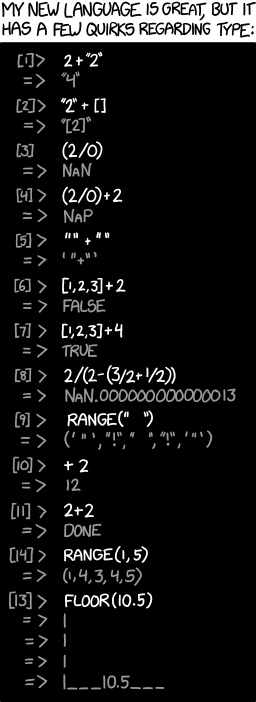
\includegraphics[width=.4\linewidth]{./gfx/xkcd-types} \\
	\enquote{\texttt{colors.rgb('{}'blue'{}')} yields \texttt{'{}'\#0000FF'{}'}.
	 \texttt{colors.rgb('{}'yellowish blue'{}')} yields \texttt{NaN}. 
	 \texttt{colors.sort()} yields \texttt{'{}'rainbow'{}'}}
	\caption[Eingabeschemata in anderen Programmiersprachen]{Eingabeschemata in anderen Programmiersprachen\newline Quelle: \url{https://xkcd.com/1537/}}
\end{figure}